% THIS IS SIGPROC-SP.TEX - VERSION 3.1
% WORKS WITH V3.2SP OF ACM_PROC_ARTICLE-SP.CLS
% APRIL 2009
%
% It is an example file showing how to use the 'acm_proc_article-sp.cls' V3.2SP
% LaTeX2e document class file for Conference Proceedings submissions.
% ----------------------------------------------------------------------------------------------------------------
% This .tex file (and associated .cls V3.2SP) *DOES NOT* produce:
%       1) The Permission Statement
%       2) The Conference (location) Info information
%       3) The Copyright Line with ACM data
%       4) Page numbering
% ---------------------------------------------------------------------------------------------------------------
% It is an example which *does* use the .bib file (from which the .bbl file
% is produced).
% REMEMBER HOWEVER: After having produced the .bbl file,
% and prior to final submission,
% you need to 'insert'  your .bbl file into your source .tex file so as to provide
% ONE 'self-contained' source file.
%
% Questions regarding SIGS should be sent to
% Adrienne Griscti ---> griscti@acm.org
%
% Questions/suggestions regarding the guidelines, .tex and .cls files, etc. to
% Gerald Murray ---> murray@hq.acm.org
%
% For tracking purposes - this is V3.1SP - APRIL 2009

\documentclass{acm_proc_article-sp}

\usepackage{caption}
\usepackage{amsmath}
\usepackage{mathtools}
\begin{document}

\title{Scalable Parallelization of Rigorous Global Optimization}


%
% You need the command \numberofauthors to handle the 'placement
% and alignment' of the authors beneath the title.
%
% For aesthetic reasons, we recommend 'three authors at a time'
% i.e. three 'name/affiliation blocks' be placed beneath the title.
%
% NOTE: You are NOT restricted in how many 'rows' of
% "name/affiliations" may appear. We just ask that you restrict
% the number of 'columns' to three.
%
% Because of the available 'opening page real-estate'
% we ask you to refrain from putting more than six authors
% (two rows with three columns) beneath the article title.
% More than six makes the first-page appear very cluttered indeed.
%
% Use the \alignauthor commands to handle the names
% and affiliations for an 'aesthetic maximum' of six authors.
% Add names, affiliations, addresses for
% the seventh etc. author(s) as the argument for the
% \additionalauthors command.
% These 'additional authors' will be output/set for you
% without further effort on your part as the last section in
% the body of your article BEFORE References or any Appendices.

\numberofauthors{3} %  in this sample file, there are a *total*
% of EIGHT authors. SIX appear on the 'first-page' (for formatting
% reasons) and the remaining two appear in the \additionalauthors section.
%
\author{
% You can go ahead and credit any number of authors here,
% e.g. one 'row of three' or two rows (consisting of one row of three
% and a second row of one, two or three).
%
% The command \alignauthor (no curly braces needed) should
% precede each author name, affiliation/snail-mail address and
% e-mail address. Additionally, tag each line of
% affiliation/address with \affaddr, and tag the
% e-mail address with \email.
%
% 1st. author
\alignauthor
Ian Briggs\\
       \email{u0692013@utah.edu}
% 2nd. author
\alignauthor
Ganesh Gopalakrishnan\\
       \email{ganesh@cs.utah.edu}
% 3rd. author
\alignauthor
Zvonimir Rakamaric\\
       \email{zvonimir@cs.utah.edu}
}
% There's nothing stopping you putting the seventh, eighth, etc.
% author on the opening page (as the 'third row') but we ask,
% for aesthetic reasons that you place these 'additional authors'
% in the \additional authors block, viz.
% Just remember to make sure that the TOTAL number of authors
% is the number that will appear on the first page PLUS the
% number that will appear in the \additionalauthors section.

\maketitle

\section{Motivation}
Floating point error is serious trouble. Graphical glitches are nothing compared to the real world cost of error, in both money and lives. The Large Hadron Collider, as costly endeavor, needed to disregard results due to an error in their floating point library \cite{bailey2013high}. Error in the Patriot missile targeting system caused 28 deaths in a single event. This accounts for $19\%$ of American soldiers killed in the Gulf War\cite{blair1992patriot}. FPTaylor is a tool for quantifying error in floating point calculations \cite{fm2015-sjrg}. The engine that drives this tool is global maximization of interval arithmetic.

\section{Introduction}
Interval arithmetic optimization has been a long held challenge in verification. Most techniques use heuristics to speed up the serial algorithm or a cooperative approach with multiple heterogenous processes\cite{alliot2012finding}. We have pushed forward in parallelizing the algorithm in a homogeneous manner to find gains in utilizing more raw computing power.

\section{Serial Algorithm}
The interval branch and bound algorithm relies on the inclusion property of interval arithmetic. Inputs to interval arithmetic operators are in the form of ranges, and the output is also a range. This range spans all possible answers from the input ranges.

To take advantage of this property the serial algorithm continually splits the input in half and examines each half for viability in the search. This is similar to a standard binary search, however both paths may be viable. The high water mark is the highest evaluation using inputs whose upper and lower bounds are the same. we know that all inputs which lead to an output with an upper bound below that high water mark cannot possibly contain the maximum. The answer variable is the highest upper bound achieved when the input ranges are thinner than a user set threshold. Local maxima become hangup points where the search continually subdivides looking at a globally unneeded path.

\section{Function Complexity}
The number of variables in the maximized function exponentially correlates to the search space. In addition the functions in question are often highly erratic, having immense numbers of local maxima.

\section{Parallel Algorithms}
The key to quick execution of this search is setting the high water mark at a high value quickly to cut off more search paths. With that in mind we have created parallel solvers to test our ideas.

\subsection{Naive Approach}
The first approach is our litmus test. All global state protected by locks. This includes the high water mark, answer, and queue of input ranges still under inquiry. Each time the high water mark updates it leads to the possibility of cutting off search paths, but at the cost of high overhead.

\subsection{Map Approach}
Instead of examining input ranges as they come out of a queue, we implemented a map based approach. The map returns a triple of nullable values; new input ranges to search, a new high water mark, and a new answer. The high water mark and answer are then updated and the new ranges mapped across. This repeats until there are no new ranges. The advantage of this is that maps are transparently parallelizable and that all search paths execute together in a lockstep fashion. This lockstep like search reduces the number of fruitless paths taken.

\subsection{Split and Overspilt Approaches}
To reduce shared state we first split the initial input range into either multiple pieces, for overspilt, or a number matching the number of threads, for split. Both then launch solvers which run to completion on their range and return a new high water mark and answer. Upon receiving an answer the main thread sends updates to worker threads if either value is greater than the main threads value. This allows for low communication traffic while still being able to aid searches still in progress. The difference with oversplit is that the worker thread is then given another range to work on until no more remain. The advantage to doing this is that a range which would go to a single worker in the split approach that has multiple local maxima becomes subdivided and given to multiple workers.  

\balancecolumns

\section{SWIG and Python}
There are interval math libraries written in C++, but to allow for quick prototyping we used Python as the main language expressing the algorithm. This leaves a gap between the computation and the algorithm which we bridged with the Simplified Wrapper and Interface Generator, SWIG\@. This allowed for python to use wrapped C++ functions for manipulating the intervals and evaluating the function. This requires that an additional source file called an interface that utilizes the header files to inform SWIG how to treat the C++ when wrapping it.

\section{Technical Challenges}
While this Python based approach yielded quick development, there were hurdles to overcome. SWIG has limited support for function overloading. For Python to pass data between processes the object must be pickleable, Python's binary serialization. This requires manual wrapping of C++ serialization in the header and interface files. Wrapped classes are not interoperable between interfaces even if the underlying C++ is the same. 

\section{Results}
The following graphs are solve times for the function $sin(x)\cdot {sin({(y\cdot z)}^2)}^{3}\cdot z+interval(3.9999999,4.000001)$. Similar speedups occur for all tested functions.

\begin{centering}
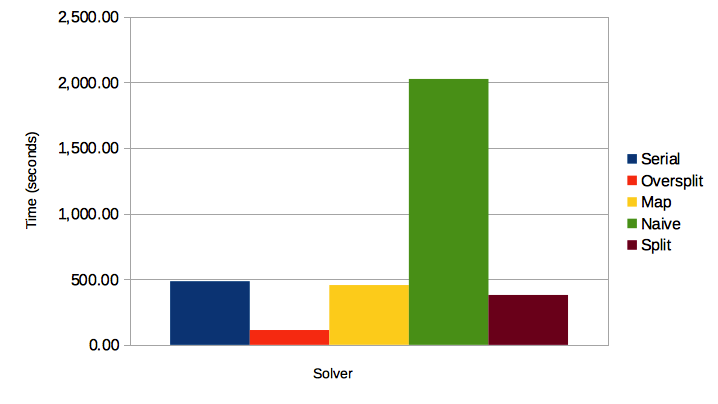
\includegraphics[width=.9\linewidth]{t1}
\captionof{figure}{Utilization of one thread}

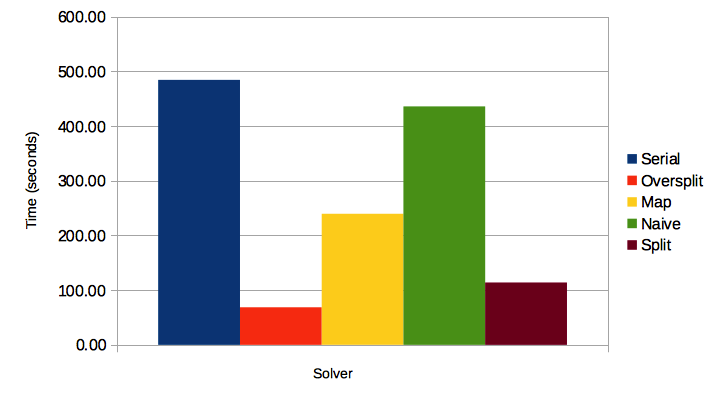
\includegraphics[width=.9\linewidth]{t44}
\captionof{figure}{Utilization of four threads}
\end{centering}

There are communication limits as the number of threads increase. This performance is tunable for each solver to produce faster results at a target thread count.

\begin{centering}
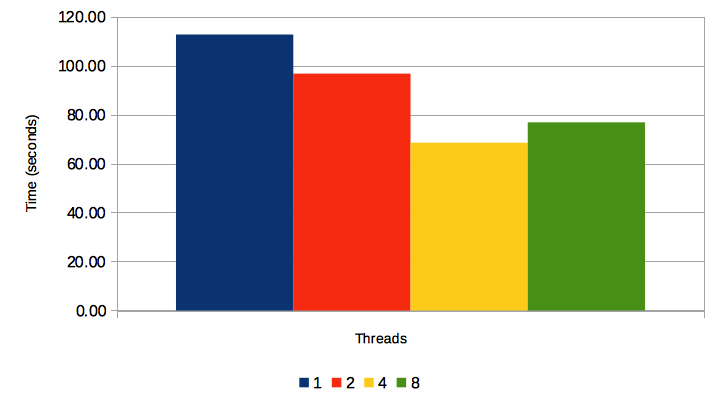
\includegraphics[width=.9\linewidth]{os}
\captionof{figure}{Thread scaling for Oversplit}

\end{centering}


\section{Future Work}
The Python implementations are only a prototyping tool and was never meant to be the end result. We are currently in the process of moving development to Rust. With the move to Rust we can race our own solver ideas against other tools.

%\end{document}  % This is where a 'short' article might terminate

%ACKNOWLEDGMENTS are optional
%
% The following two commands are all you need in the
% initial runs of your .tex file to
% produce the bibliography for the citations in your paper.
%\nocite{*} % Insert publications even if they are not cited in the poster
\bibliographystyle{abbrv}
\bibliography{sigproc}  % sigproc.bib is the name of the Bibliography in this case
% You must have a proper ".bib" file
%  and remember to run:
% latex bibtex latex latex
% to resolve all references
%
% ACM needs 'a single self-contained file'!
%
%APPENDICES are optional
\balancecolumns



%\balancecolumns
% That's all folks!
\end{document}
